%! Author = breandan
%! Date = 2/22/21

% Preamble
\documentclass[11pt]{article}

% Packages
\usepackage{amsfonts}
\usepackage{amsmath}
\usepackage{graphicx}
\usepackage{hyperref}
\usepackage{float}

% Document

\title{Learning to navigate, read and apply\\software documentation like a human}
\author{Breandan Considine, Xujie Si, Jin Guo}
\begin{document}
\maketitle

\section{Introduction}

Humans are adept information foraging agents. We can quickly find relevant information in a large corpus by recognizing and following textual landmarks. Software projects are composed of a variety of semi-structured documents containing many such clues where relevant information may be found. In this work, we train an agent to navigate and read software artifacts like source code and documentation, in order to facilitate common programming tasks such as code completion or defect prediction.

%Our work broadly falls under the umbrella of text-based reinforcement learning. Prior literature falls under two categories: natural or formal language. Reinforcement learning (RL) in the natural domain typically focuses on question answering~\cite{buck2017ask, chen2019reinforcement}, or interactive text games~\cite{he2015deep,ammanabrolu2018playing,narasimhan2015language,guo2020interactive,ammanabrolu2020graph}. RL techniques have begun to show promising results for program synthesis~\cite{ellis2019write, johnson2020learning, chen2020program}. Our work falls at the intersection of these two domains.

Early work in program learning realized the importance of graph-based representations~\cite{allamanis2017learning}, however explicit graph construction requires extensive feature-engineering. More recent work in program synthesis has explored incorporating a terminal~\cite{ellis2019write}, graphical~\cite{walke2020learning} or other user interface to explore the space of valid programs, however do not consider the scope or variety of artifacts in a software project. Adapting to settings where style, terminology and document structure vary remains a challenge. Early work has shown the feasibility of learning a graph~\cite{johnson2020learning} from source code, but only locally and still requires an explicit parser to form the initial graph.

%Unlike prior work, we consider the whole project and related artifacts. Instead of parsing their contents explicitly, which may be computationally expensive or too large to fit in memory, we allow the agent to construct the graph organically by exploring the filesystem, which can later be used to predict a label or sequence at inference time, depending on the task.

Imagine a newly-hired developer, who has programming experience, but no prior knowledge about a closed-source project. She receives access to the team's Git repository and is assigned her first ticket: Fix test broken by \texttt{0fb98be}. After locating the commit and becoming familiar with the code, she queries StackOverflow, discovers a relevant solution, copies the code into the project, makes a few edits, presses run, and the test passes.

In order to accomplish a similar task, an information-seeking agent must be able to explore a database. Similar to a human developer, it might be able to perform simple actions, like \texttt{search(query)}, \texttt{read(text)}, \texttt{copy(text, from, to)}, and \texttt{runCode()} while navigating relevant documents and source code artifacts. As the agent traverses the project using these primitives, it builds up a project-specific knowledge graph.

%\begin{figure*}
%  \centering
%  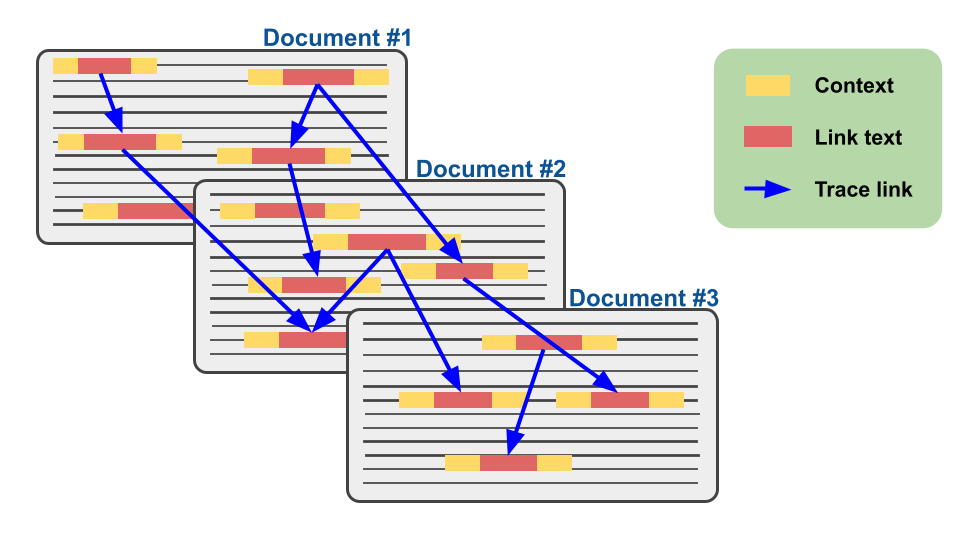
\includegraphics[width=0.8\textwidth]{use_graph}
%  \caption{Software projects consist of many documents which share common references. These references form an entity alignment graph, with vertices decorated by the surrounding context, and edges by the relation type, e.g. exact duplicate, fuzzy match or synthetic relation (learned or engineered).}
%\end{figure*}

%During evaluation, we measure task performance across search strategies. Depending on the task in question, various loss functions are possible, from a simple string distance metric over a masked code fragment, to more complex properties (e.g. the presence or absence of errors, or some internal state of the REPL) that must be satisfied by interacting with the runtime environment. Many program analysis and repair tasks are also possible, such as defect, duplicate or vulnerability detection and correction.

\section{Method}



We fetch a dataset of repositories sampled from popular Java repositories on GitHub, containing a mixture of filetypes representing source code and natural language artifacts. From each repository, we index all substrings of every line in every file using a variable height radix tree producing a multimap of $\texttt{kwdIndex: String -> List<Location<F, O>>}$ of $\texttt{String}$  queries to file-offset pairs. We also encode CodeBERT~\cite{feng2020codebert} sequence embeddings to substrings $\texttt{knnIndex: Vector -> Location<F, O>}$ using a Hierarchial Navigavble Small World Graph~\cite{malkov2018efficient} (HNSWG).


\begin{figure}[H]
  \centering
  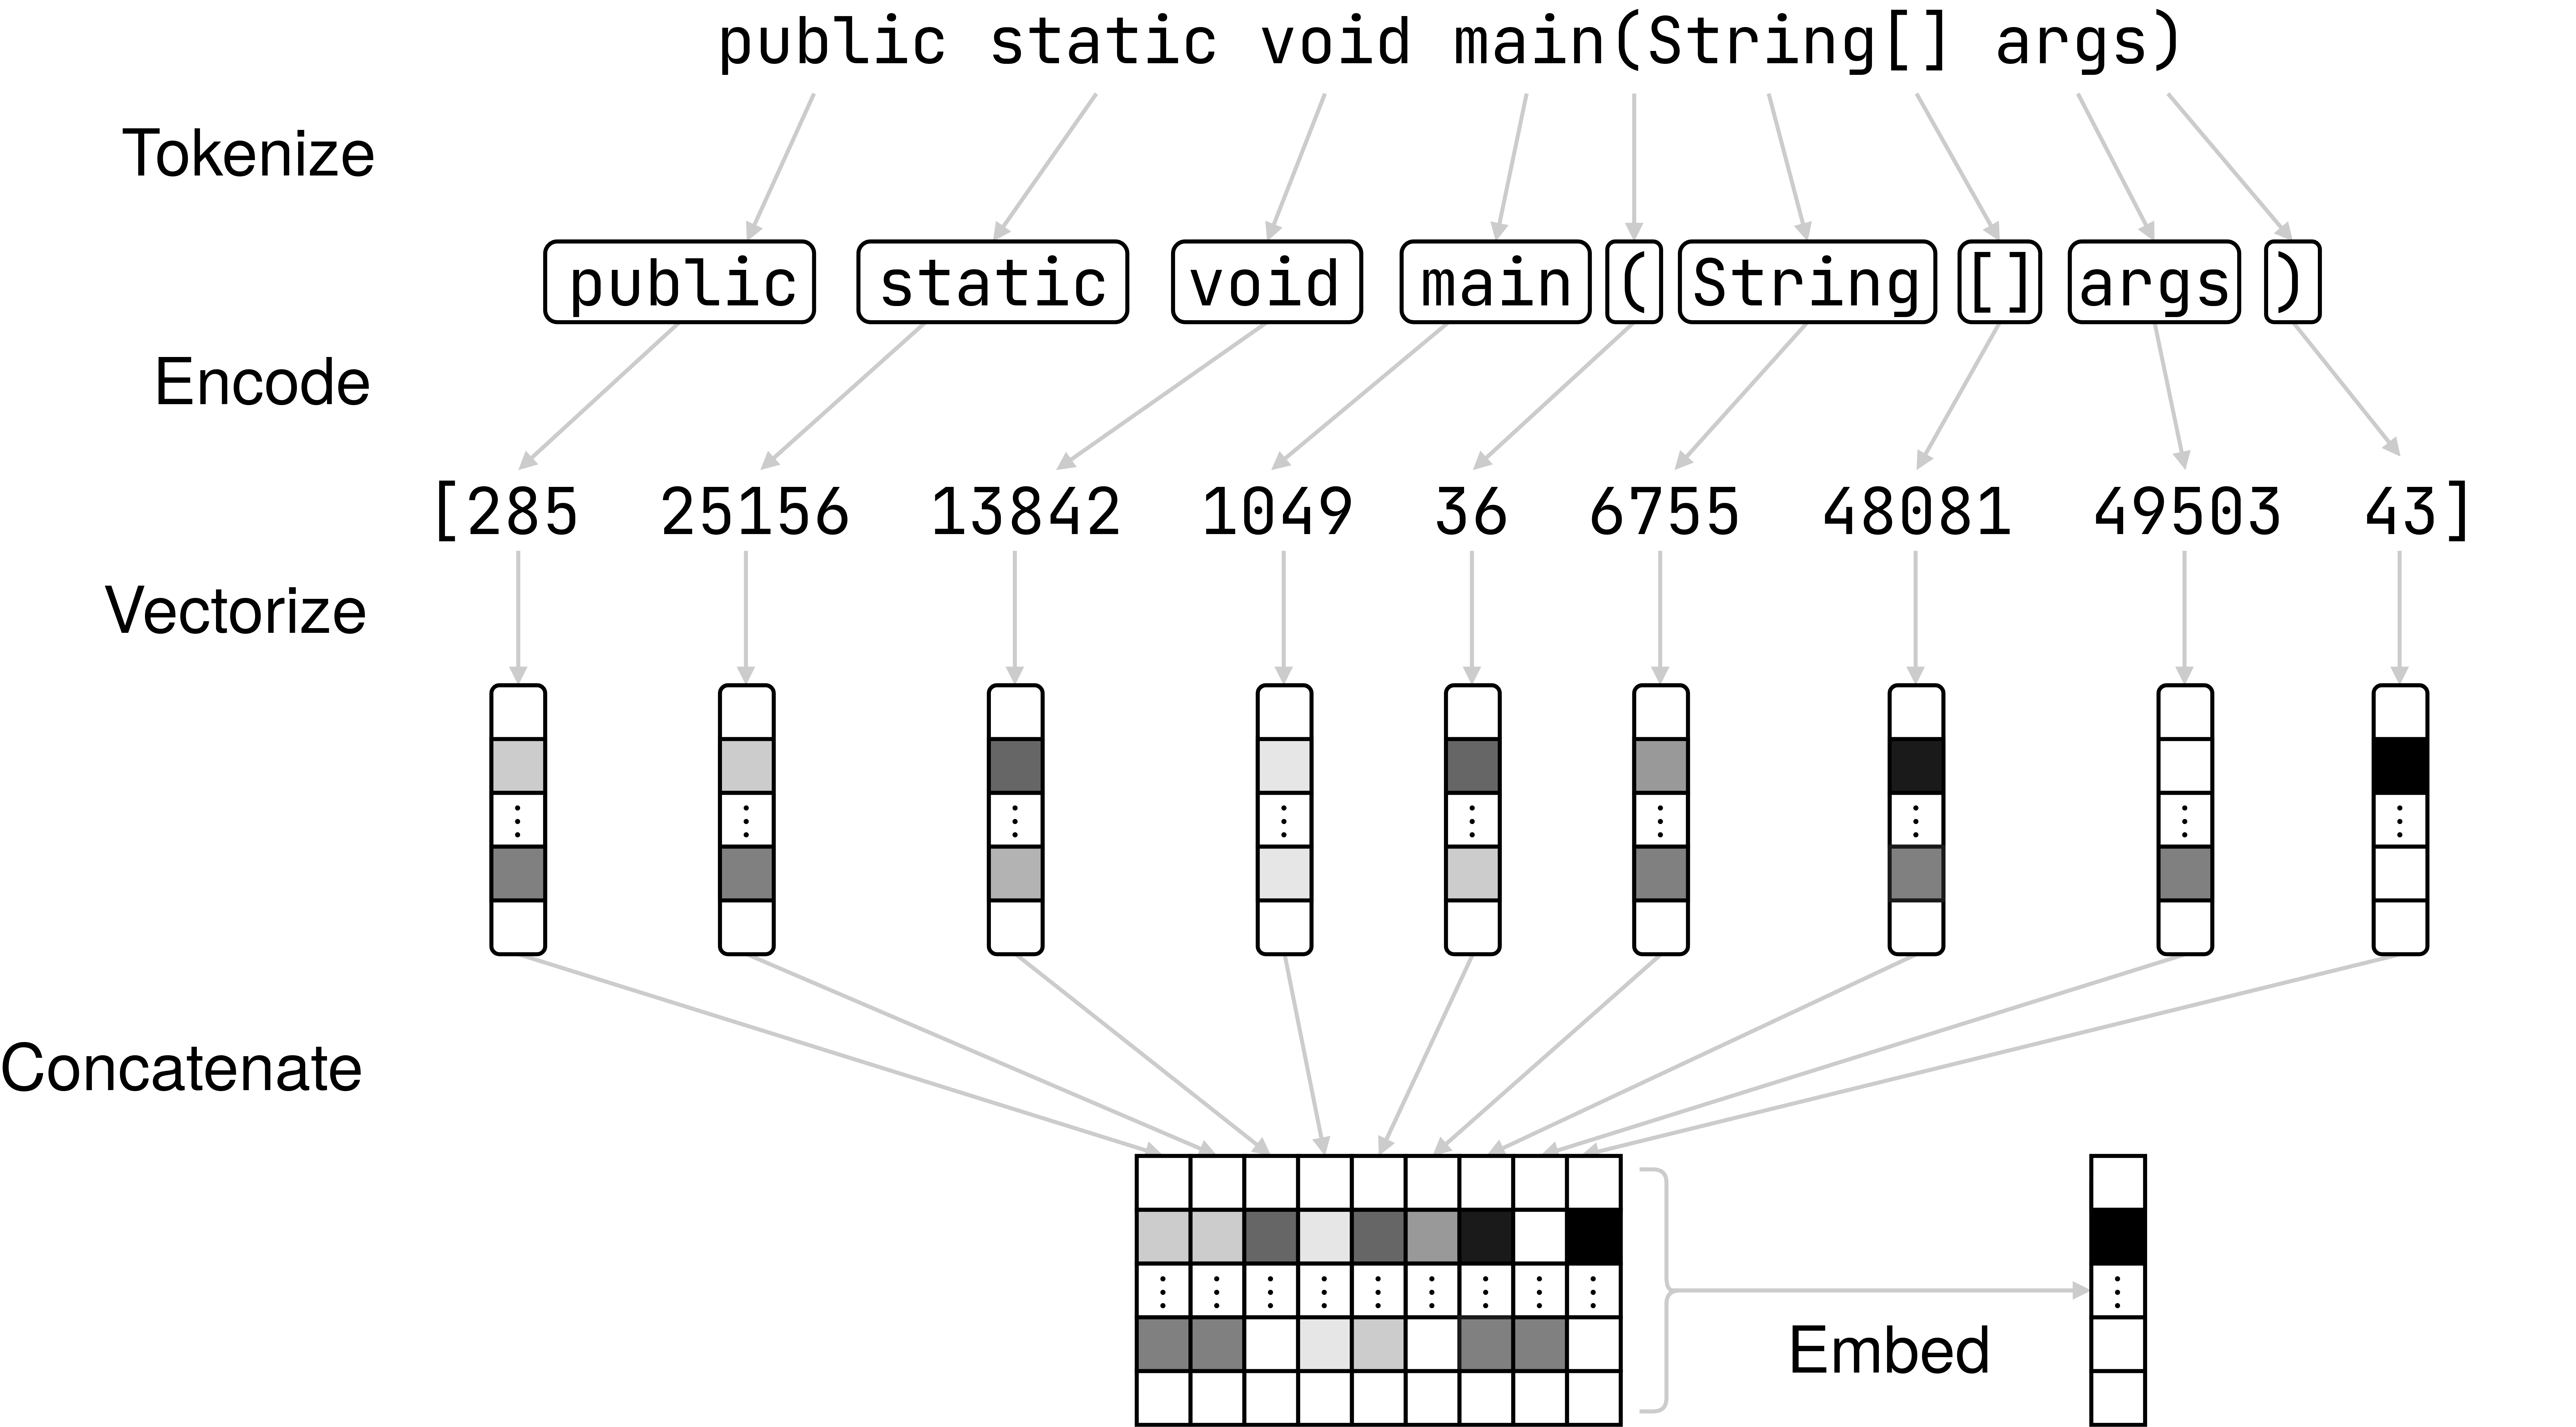
\includegraphics[width=0.85\textwidth]{bert_embedding}
  \caption{CodeBERT takes a unicode sequence and emits a vector sequence, which we accumulate into a single vector.}
\end{figure}

For each token in a string, CodeBERT emits a length-512 vector, so a line with $n$ tokens produces a matrix of shape $\mathbb R^{512\times n}$, which we flatten into a vector. Once we have the sequence-embedding, we compare various distance-metrics to fetch the nearest sequence embeddings in our database. We then compare precision and recall across various types of distance metrics.

\begin{figure}[H]
  \centering
  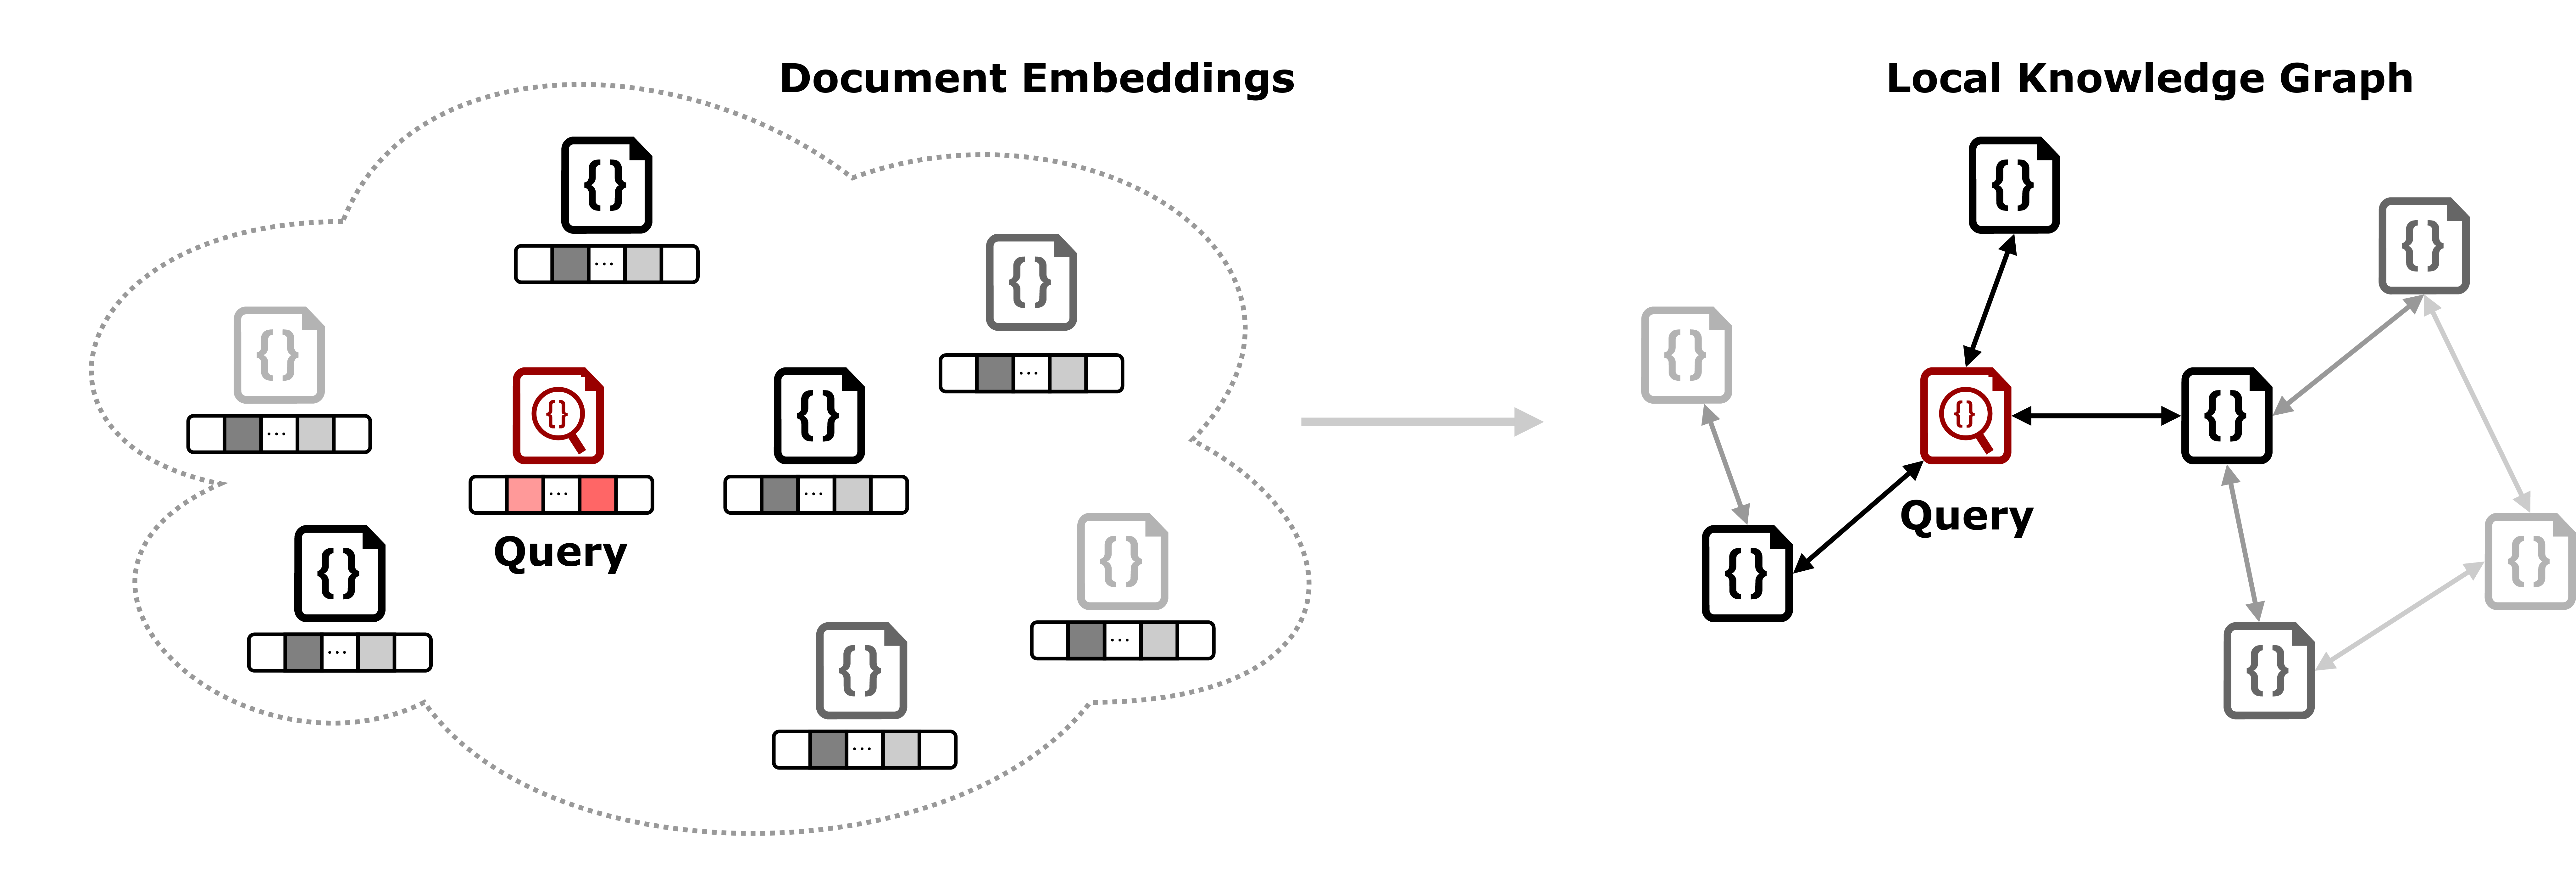
\includegraphics[width=0.85\textwidth]{latent_kg}
  \caption{To compute the k-nearest neighbors for a given query, we traverse the HNSWG up to depth $d$, i.e. $d=2$ retrieves the neighbors-of-neighbors, and $d=3$ fetches the neighbors-of-neighbors-of-neighbors.}
\end{figure}

For a given query location, we compute the context embedding and fetch the k-nearest neighboring documents in latent space. The edges are decorated with the direction vector between neighbors. We then repeat the procedure recursively, pruning with a beam search heuristic based on the path length the latent space.

\begin{figure}[H]
  \centering
  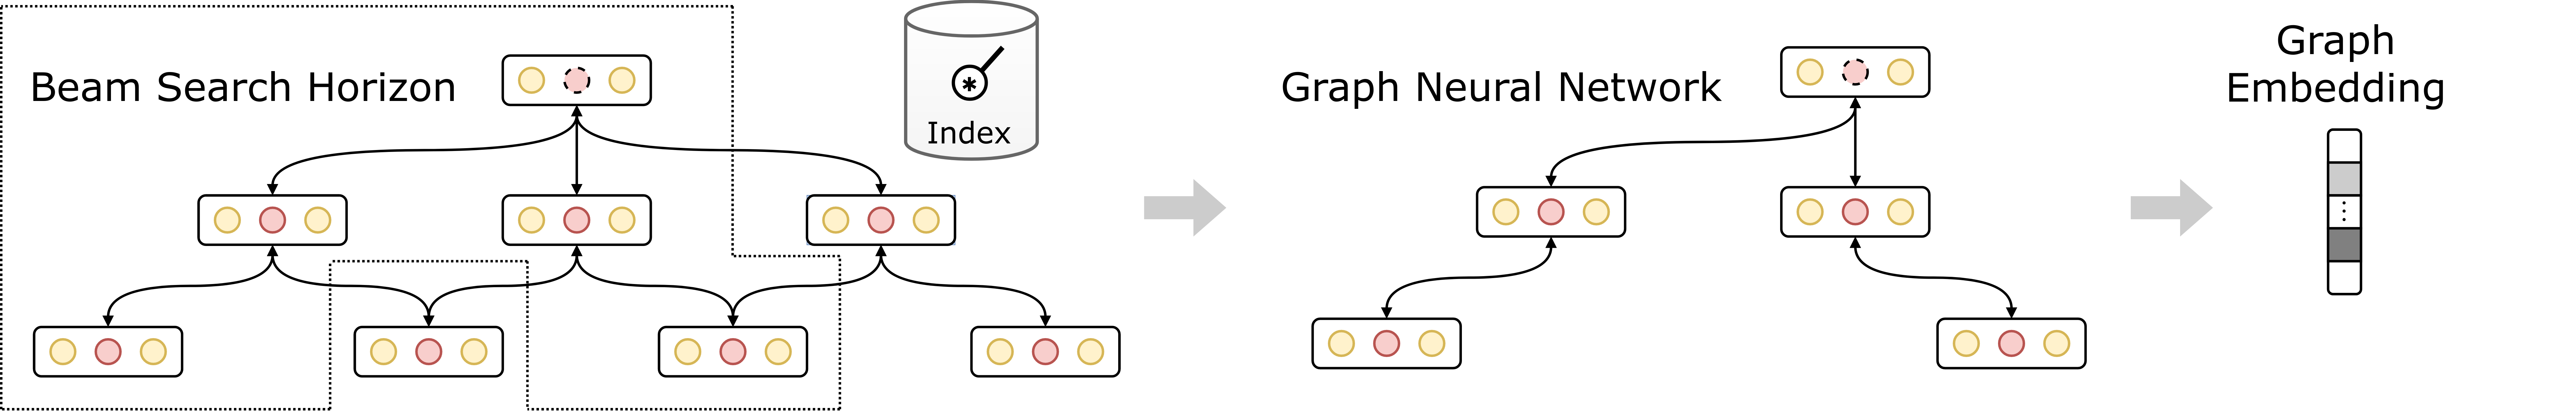
\includegraphics[width=1.05\textwidth]{architecture}
  \caption{Unlike language models which directly learn the data distribution, our model is designed to query an unseen database only available at test time. The model scores and selectively expands a subset of promising results within the database using a beam search heuristic, then runs message passing over the resulting graph to obtain the final task prediction.}
\end{figure}

Once the beam search procedure is complete, we have a graph of the nearest neighboring documents. This forms a virtual knowledge graph, with nodes decorated by the CodeBERT embeddings and edges decorate with the direction vector between the documents. We then run $p$ rounds of message passing to generate a neighborhood summary.

% We initialize the policy network using a pretrained language model. Starting at the site of the prediction task and conditioning on its local context, the policy network draws K queries from its latent state, which are fed into the index to produce a set of matching locations. The model scores and selectively expands a subset of those locations, and the process is repeated using finite-horizon MCTS or similar beam search procedure to retrieve a set of contextually relevant locations within the parent project.
%
%The rollout traces form a graph of related locations inside each project and their corresponding context embeddings, which together form the GNN node features. Once the rollout ends, we run message passing on the resulting GNN for a fixed numbers of steps and decode the graph embedding to obtain a task prediction. The decoder, GNN parameters, and policy network are all trained end-to-end on the downstream task, e.g. code completion, defect detection or correction. After convergence, we compare the results across horizon size and analyze the queries and filetypes which are selected.

\section{Experiments}

In this work, we attempt to understand the relationship between entities in a software project. Our research seeks to answer the following questions:

\begin{enumerate}
  \item Which contexts in a software project share mutual information?
  \item To what degree can we claim the agent has learned to:\begin{enumerate}
  \item Locate contextually relevant artifacts within a software project?
  \item Comprehend the semantic content of the artifacts traversed?
  \item Apply the knowledge gathered to perform the assigned task?
  \end{enumerate}
\end{enumerate}

In contrast with classical code completion models which only require a file-local context, our method is designed to navigate an entire project. In the following experiments, we compare completion accuracy with a vanilla sequence prediction model, as well as an AST-structured sequence prediction model trained from a corpus of Java projects on the same task.

We hypothesize that by jointly learning to choose locations in a project over which to attend while solving a downstream task, such as masked sequence completion, our model will produce a feature representation capable of locating and extracting information from semantically relevant locations. We evaluate our hypothesis both qualitatively and quantitatively.

In our first experiment, we attempt to understand which queries the agent is performing while solving a programming task. Does it search for certain keywords in the context? Are those keywords relevant to the task?

In our second experiment, we try to understand the approximate relation between project artifacts and measure the information gain from various filetypes through ablation. For trajectories containing filetypes which include Markdown or Java, what kinds of information do these resources provide and which categories are most salient for the assigned prediction task?

In our third experiment, we compare prediction accuracy across architectures and datasets. Should we constrain the action space (e.g. only querying tokens from the surrounding context) for more efficient trajectory sampling, or allow arbitrary queries? How well does the model architecture transfer to new repositories, within and across programming languages?

If our hypothesis is correct, the policy network will learn to use both natural language and source code artifacts. If so, this would provide evidence to support the broader hypothesis~\cite{guo2017semantically} that documentation is a useful source of information. In addition to being useful for the prediction task itself, we anticipate our model could also be used for knowledge graph extraction.


\section{Next steps}

Our next steps are to build a simple RL environment which allows an agent to interact with a software repository and construct a graph. We will use an in-memory filesystem to store and load project artifacts. The policy network will need to be pretrained on a corpus of projects in the same language. To model the action space, we will use the radix tree of the parent project, with transition probabilities conditioned on the local context.

For further details and to get started, please visit our GitHub page: \url{https://github.com/breandan/gym-fs}.

\section{Results}

  \bibliography{research_proposal}
  \bibliographystyle{plain}
\end{document}